\chapter{Theory} \label{sec:theory}
\section{Acoustical properties of ultrasound}

\begin{figure}[ht]
	\centering
	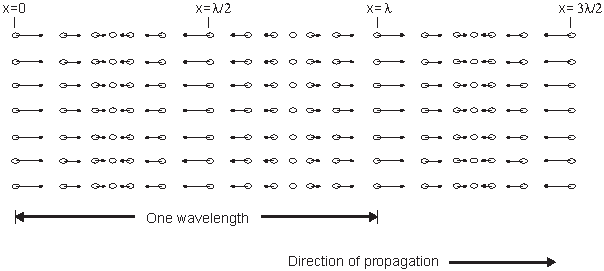
\includegraphics[width=.6\textwidth]{1_plane_wave_jensen-cropped.pdf}
	\caption{Particle displacement for a propagating ultrasound wave \cite{JensenUltrasoundBook}}
	\label{fig:1_planewave_jensen}
\end{figure}

Ultrasound is a technology that transmit sound wave with frequencies above the audible range (\qtyrange[range-units = single]{20}{20e3}{\hertz}) to mechanically vibrate matter. The particles in the medium would be at rest and distributed uniformly before any disturbance. The wave propagates as a disturbance and the particles oscillate around their mean position due to the presence of the ultrasonic wave. Typically the \glsxtrshort{US} frequency band used in clinical settings are from \qtyrange[range-units = single]{2}{12}{\mega\hertz}. \Cref{fig:1_planewave_jensen} visualizes the propagation of a plane wave in matter. The oscillation occurs parallel to the wave's direction, making it longitudinal, and the disturbance will propagate with the variable $c$, which is determined by the medium and is given by \cref{eq:1_velocity_c}.
\begin{equation} \label{eq:1_velocity_c}
	c = \sqrt{\frac{1}{\rho_{0} \kappa_{S}}}
\end{equation}
Where $\rho_{0}$ is the mean density (\si{\kilogram\per\meter\cubed}) and $\kappa_{S}$ is the \gls{adiabatic} compressibility (\si{\meter\squared\per\newton}). Since in the majority of cases, the propagation of ultrasound is linear, it is assumed in this work. 

The acoustic pressure of the harmonic plane wave is expressed by \cref{eq:1_acoustic_pressure}
\begin{equation} \label{eq:1_acoustic_pressure}
	p(t,z)=p_{0} e^{j(\omega t - k z)}
\end{equation}
And propagates along the $z$-axis. $\omega$ is the angular frequency, $k$ is the wave number and is expressed by $k=\nicefrac{\omega}{c}=\nicefrac{2\pi}{\lambda}$, and $_{0}$ is the acoustic pressure amplitude. A spherical wave is expressed by \cref{eq:1_spherical_wave}
\begin{equation} \label{eq:1_spherical_wave}
	p(t,r)=p_{0} e^{j(\omega t - k r)}
\end{equation}
Where $r$ is radial distance, and is defined in a polar coordinate system. For each time instance, the acoustic pressure $p(t,r)$ is constant over a fixed radial position. In this scenario, the pressure amplitude is given by $p_{0}(r) = \nicefrac{k_{p}}{r}$, where $k_{p}$ is a constant since the energy of the outgoing wave must be constant.  Particle speed $u$ is dependent on the pressure caused by a wave expressed by \cref{eq:1_particle_speed}
\begin{equation} \label{eq:1_particle_speed}
	u = \frac{p}{Z}
\end{equation}
Where $Z$ is the characteristic acoustic impedance, defined as the ratio of acoustic pressure to particle speed at a given position in the medium and is expressed by \cref{eq:1_acoustic_impedance}.
\begin{equation} \label{eq:1_acoustic_impedance}
	Z = \rho_{0} c
\end{equation}

Characteristic acoustic impedance $Z$ is one of the most significant variables in the characterization of propagating plane waves. Reference values for density, speed of sound, and characteristic acoustic impedance can be seen in \cref{tab:density_tissue}.

\begin{table}[ht]
	\centering
	\sisetup{range-phrase=--,range-exponents = combine}
	\begin{tabularx}{\linewidth}{@{}lSSS@{}}
		\toprule
		\textbf{Medium}          & {\makecell{\textbf{Density}\\\unit[per-mode = symbol]{\kilogram\per\meter\cubed}}} & {\makecell{\textbf{Speed of sound}\\\unit[per-mode = symbol]{\meter\per\second}}} & {\makecell{\textbf{Characteristic}\\\textbf{acoustic impedance}\\\unit[per-mode = symbol]{\kilogram\per\meter\squared\per\second}}} \\ \midrule
		Air             & 1.2     & 333            & 0.4e3       \\
		Blood           & 1.06e3    &    1566        &  1.66e6     \\
		Bone            & \numrange{1.38e3}{1.81e3}  &   \numrange{2070}{5350}{}       & \numrange{3.75e6}{7.38e6}{} \\
		Brain           &  1.03e3       & \numrange{1505}{1612}{}  & \numrange{1.55e6}{1.66e6}{} \\
		Fat             &  0.92e3  &  1446 & 1.33e6 \\
		Kidney          &  1.04e3  & 1567 & 1.62e6 \\
		Lung            &  0.4e3  &  650  & 0.26e6 \\
		Liver           &  1.06e3  &  1566  & 1.66e6 \\
		Muscle          &  1.07e3  & \numrange{1542}{1626}{} & \numrange{1.65e6}{1.74e6}{} \\
		Spleen          &  1.06e3  & 1566 & 1.66e6 \\
		Distilled water &  1e3  & 1480 & 1.48e6 \\ \bottomrule
	\end{tabularx}
	\caption{Approximate density, sound speed, and acoustic impedance of human tissue types \cite{JensenUltrasoundBook}}
	\label{tab:density_tissue}
\end{table}

In the following sections, various acoustic wave phenomena will be briefly described.

\subsection{Scattering}
A wave propagating across a medium continues in the same direction until it encounters a new medium. When this occurs, a portion of the wave is transmitted into the new medium, with a change in direction. Because the scattered wave is the result of several contributors, it is necessary to define it statistically. The amplitude distribution is Gaussian \cite{JensenUltrasoundBook} and can thus be fully described by its mean and variance. The mean value is zero because the dispersed signal is caused by variances of the acoustic characteristics in tissue.

The correlation between multiple data is what allows ultrasound to determine blood velocities.
Because minor movements have a significant correlation, it is feasible to discover alterations in location by comparing sequential measurements of moving structure, such as blood cells. In medical ultrasound, just one transducer is utilised for transmitting and receiving, and only the backscattered signal is analysed. 

The power of scattered signal is defined by the scattering cross-section, which in small cases mean a uniform intensity $I_{i}$, and is expressed by \cref{eq:1_scatter_power}.

\begin{equation} \label{eq:1_scatter_power}
	P_{s} = I_{i} \sigma_{s c}
\end{equation}
Where $\sigma_{s c}$ is the scattering cross-section. 

\subsection{Attenuation}

\subsection{Transducer}

\begin{figure}[ht]
	\centering
	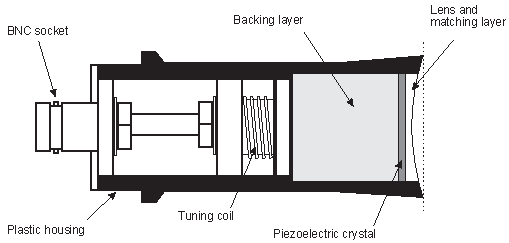
\includegraphics[width=.6\textwidth]{1_transducer_construction-cropped.pdf}
	\caption{Single element ultrasound transducer construction \cite{JensenUltrasoundBook}}
	\label{fig:1_transducer_construction}
\end{figure}

A layperson knows transducers as speakers and microphones in the context of PA systems. In the case of medical ultrasound it is the device that generates the acoustic pressure field, which is emitted into tissue. The transducer has a piezoelectric crystal inside the housing. When excited, this crystal emits ultrasound waves toward flowing blood. The red blood cells will reflect a fraction of the emitted waves. These reflected waves are of a different frequency than the transmitted wave. If the red blod cells are moving away from the transducer, the frequency will be lower. If the red blod cells are moving towards the transducer, the frequency will be higher. This is caused by the \gls{doppler}. The reflected ultrasonic waves return to the crystal and are converted back into electrical signals. The single element transducer shown in \cref{fig:1_transducer_construction} has a minimal imaging window and has to be mechanically manipulated to get a wide window, which is unfeasible for responsive high-frequency imaging. Thus, usually an array transducer is used. Various ultrasound transducer types exist with different strengths and weaknesses, shown in \cref{fig:1_transducer_types}. 

\begin{figure}[ht]
	\centering
	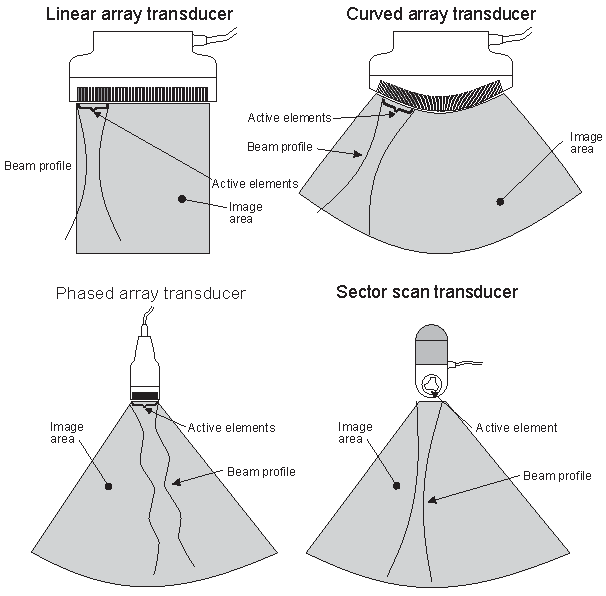
\includegraphics[width=.6\textwidth]{1_transducer_types-cropped.pdf}
	\caption{Single element ultrasound transducer construction \cite{JensenUltrasoundBook}}
	\label{fig:1_transducer_types}
\end{figure}

\begin{figure}[ht]
	\centering
	\resizebox{\textwidth}{!}{
		%\begin{tikzpicture}
%	[outer sep=0,
%>=latex,
%align=center]
%% Draw nodes
%\node[place]		(human_in)	[draw=none]											{Control\\input};
%\node[place]		(embed)		[inner sep=1mm,rectangle,right=10mm of human_in]	{Control\\system};
%\node[place]		(wave_gen)		[inner sep=1mm,rectangle,right=5mm of embed]			{Pulse\\generator};
%\node[place]		(pwr_stg)	[inner sep=1mm,rectangle,right=5mm of wave_gen]	{Power\\stage};
%\node[place]		(tr_switch)	[inner sep=1mm,rectangle,right=5mm of pwr_stg]	{T/R\\switch};
%\node[place]		(transducer)		[inner sep=1mm,rectangle,right=5mm of tr_switch]	{Transducer};
%\node[place]		(preamp)		[inner sep=1mm,rectangle,below=5mm of tr_switch]	{Preamplifier};
%\node[place]		(bpf)		[inner sep=1mm,rectangle,below=5mm of preamp]	{BPF};
%\node[place]		(demod)		[inner sep=1mm,rectangle,left=10mm of bpf]		{Demodulator};
%\node[place]		(lpf1)		[inner sep=1mm,rectangle,above=5mm of demod]		{LPF 1};
%\node[place]		(lpf2)		[inner sep=1mm,rectangle,below=5mm of demod]		{LPF 2};
%\node[place]		(sha1)		[inner sep=1mm,rectangle,left=5mm of lpf1]		{SHA 1};
%\node[place]		(sha2)		[inner sep=1mm,rectangle,left=15mm of lpf1]		{SHA 2};
%
%% Draw lines between nodes
%\draw [|->] 		(human_in) 		to 		(embed);
%\draw [->]			(embed)			to		(wave_gen);
%\draw [->]			(wave_gen)		to		(pwr_stg);
%\draw [->]			(pwr_stg)		to		(tr_switch);
%\draw [<->]			(tr_switch)		to		(transducer);
%\draw [->]			(tr_switch)		to		(preamp);
%\draw [->]			(preamp)		to		(bpf);
%\draw [->]			(bpf)		to		(demod);
%\draw [->]			(demod)		to		(lpf1);
%\draw [->]			(demod)		to		(lpf2);
%\draw [-|>]			(lpf1)		to		(sha1);
%\draw [-|>]			(lpf2)		to		(sha2);
%\draw [-|>]			(sha1)		to		(embed);
%\draw [-|>]			(sha2)		to		(embed);
%
%% Draw rectangle
%\draw[draw=black,dashed,red] (13mm,8mm) rectangle ++(45mm,-15mm);
%\end{tikzpicture}
%\begin{tikzpicture}
%	[outer sep=0,
%	>=latex,
%	align=center,
%	line width = 1pt,
%	% on grid,
%	start chain = going right,
%	node distance = 5cm,
%	%box/.style = {draw, rectangle, font=\huge, on chain},
%	box/.style = {draw, rectangle, on chain},
%	%L/.style = {draw, red, -{Stealth[scale=3,length=3,width=2]}},
%	L/.style = {draw, -{Stealth[scale=3,length=3,width=2]}},
%	%T/.style = {draw, red, rounded corners,
%		T/.style = {draw, rounded corners,
%			to path={-| (\tikztotarget)},
%			-{Stealth[scale=3,length=3,width=2]}}]
%
%		% Draw nodes
%		\node[place]		(human_in)	[draw=none]											{Control\\input};
%		\node[place]		(embed)		[inner sep=1mm,rectangle,right=10mm of human_in]	{Control\\system};
%		\node[place]		(wave_gen)		[inner sep=1mm,rectangle,right=5mm of embed]			{Pulse\\generator};
%		\node[place]		(pwr_stg)	[inner sep=1mm,rectangle,right=5mm of wave_gen]	{Power\\stage};
%		\node[place]		(tr_switch)	[inner sep=1mm,rectangle,right=5mm of pwr_stg]	{T/R\\switch};
%		\node[place]		(transducer)		[inner sep=1mm,rectangle,right=8mm of tr_switch]	{Transducer};
%		\node[place]		(preamp)		[inner sep=1mm,rectangle,below=5mm of tr_switch]	{Preamplifier};
%		\node[place]		(bpf)		[inner sep=1mm,rectangle,below=5mm of preamp]	{BPF};
%		\node[place]		(demod)		[inner sep=1mm,rectangle,left=10mm of bpf]		{Demodulator};
%		\node[place]		(lpf2)		[inner sep=1mm,rectangle,above=5mm of demod]	{LPF 2};
%		\node[place]		(lpf1)		[inner sep=1mm,rectangle,left=5mm of demod]		{LPF 1};
%		\node[place]		(sha2)		[inner sep=1mm,rectangle,left=10mm of lpf2]		{SHA 2};
%		\node[place]		(sha1)		[inner sep=1mm,rectangle,left=27.5mm of lpf2]		{SHA 1};
%
%		% Draw lines between nodes
%		\draw [L,|->] 		(human_in) 		to 		(embed);
%		\draw [L,->]			(embed)			to		(wave_gen);
%		\draw [L,->]			(wave_gen)		to		(pwr_stg);
%		\draw [L,->]			(pwr_stg)		to		(tr_switch);
%		\draw [L,<->]			(tr_switch)		to		(transducer);
%		\draw [L,->]			(tr_switch)		to		(preamp);
%		\draw [L,->]			(preamp)		to		(bpf);
%		\draw [L,->]			(bpf)		to		(demod);
%		\draw [L,->]			(demod)		to		(lpf1);
%		\draw [L,->]			(demod)		to		(lpf2);
%		\draw [T,->]			(lpf1)		to		(sha1);
%		\draw [L,->]			(lpf2)		to		(sha2);
%		\draw [T,->]			(sha1)		to		(embed);
%		\draw [T,->]			(sha2)		to		(embed);
%
%		% Draw rectangle
%		%\draw[draw=black,dashed,red] (13mm,8mm) rectangle ++(45mm,-15mm);
%	\end{tikzpicture}
\begin{tikzpicture}
	[outer sep=0,
	>=latex,
	align=center,
	line width = 1pt,
	% on grid,
	start chain = going right,
	node distance = 5cm,
	%box/.style = {draw, rectangle, font=\huge, on chain},
	box/.style = {draw, rectangle, on chain},
	%L/.style = {draw, red, -{Stealth[scale=3,length=3,width=2]}},
	L/.style = {draw, -{Stealth[scale=3,length=3,width=2]}},
	%T/.style = {draw, red, rounded corners,
		T/.style = {draw, rounded corners,
			to path={-| (\tikztotarget)},
			-{Stealth[scale=3,length=3,width=2]}}]

		% Draw nodes
		\node[place]		(human_in)	[draw=none]											{Control\\input};
		\node[place]		(embed)		[inner sep=1mm,rectangle,right=10mm of human_in]	{Control\\system};
		\node[place]		(wave_gen)		[inner sep=1mm,rectangle,right=5mm of embed]			{Pulse\\generator};
		\node[place]		(pwr_stg)	[inner sep=1mm,rectangle,right=5mm of wave_gen]	{Power\\stage};
		\node[place]		(tr_switch)	[inner sep=1mm,rectangle,right=5mm of pwr_stg]	{T/R\\switch};
		\node[place]		(transducer)		[inner sep=1mm,rectangle,right=10mm of tr_switch]	{Transducer};
		\node[place]		(preamp)		[inner sep=1mm,rectangle,below=5mm of tr_switch]	{Preamplifier};
		\node[place]		(bpf)		[inner sep=1mm,rectangle,below=5mm of preamp]	{BPF};
		\node[place]		(demod)		[inner sep=1mm,rectangle,left=5mm of bpf]		{Demodulator};
		%\node[place]		(lpf2)		[inner sep=1mm,rectangle,above=5mm of demod]	{LPF 2};
		\node[place]		(lpf1)		[inner sep=1mm,rectangle,left=5mm of demod]		{LPF};
		%\node[place]		(sha2)		[inner sep=1mm,rectangle,left=10mm of lpf2]		{SHA 2};
		\node[place]		(sha1)		[inner sep=1mm,rectangle,left=5mm of lpf1]		{SHA};
		\node[place]		(hpf)		[inner sep=1mm,rectangle,above=5mm of sha1]		{HPF};

		% Draw lines between nodes
		\draw [L,|->] 		(human_in) 		to 		(embed);
		\draw [L,->]			(embed)			to		(wave_gen);
		\draw [L,->]			(wave_gen)		to		(pwr_stg);
		\draw [L,->]			(pwr_stg)		to		(tr_switch);
		\draw [L,<->]			(tr_switch)		to		(transducer);
		\draw [L,->]			(tr_switch)		to		(preamp);
		\draw [L,->]			(preamp)		to		(bpf);
		\draw [L,->]			(bpf)		to		(demod);
		\draw [L,->]			(demod)		to		(lpf1);
		%\draw [L,->]			(demod)		to		(lpf2);
		\draw [L,->]			(lpf1)		to		(sha1);
		%\draw [L,->]			(lpf2)		to		(sha2);
		\draw [L,->]			(sha1)		to		(hpf);
		%\draw [T,->]			(sha2)		to		(embed);
		\draw [L,->]			(hpf)		to		(embed);

		% Draw rectangle
		%\draw[draw=black,dashed,red] (13mm,8mm) rectangle ++(45mm,-15mm);
	\end{tikzpicture}
	}
	\caption{Simple overview of the system}
	\label{fig:1_system_overview}
\end{figure}


